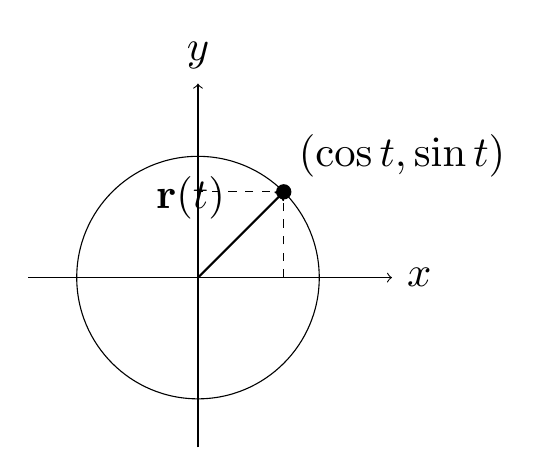
\begin{tikzpicture}[scale=1.54, transform shape]
    \draw[->] (-1.4,0) -- (1.6,0) node[right] {$x$};
    \draw[->] (0,-1.4) -- (0,1.6) node[above] {$y$};
    \draw (0,0) circle (1);
    \draw[->, thick] (0,0) -- ({cos(45)},{sin(45)}) node[midway, above left] {$\mathbf{r}(t)$};
    \fill ({cos(45)},{sin(45)}) circle (1.8pt);
    \draw[dashed] ({cos(45)},0) -- ({cos(45)},{sin(45)}) -- (0,{sin(45)});
    \node[above right] at ({cos(45)},{sin(45)}) {$(\cos t,\sin t)$};
\end{tikzpicture}
